\documentclass{article}

\usepackage{tikz}
\usetikzlibrary{automata,positioning}
\begin{document}

\centering
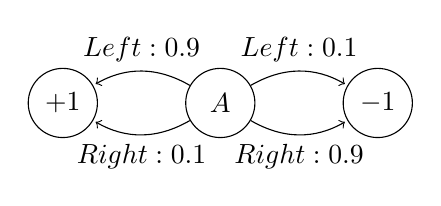
\begin{tikzpicture}[shorten >=1pt,node distance=2cm,on grid,auto] 
   \node[state] (2)   {$A$}; 
   \node[state](3) [left=of 2] {$+1$};
   \node[state](1) [right=of 2] {$-1$};
    \path[->] 
    (2) edge[bend right]  node[pos=0.5, sloped, above]  {$Left: 0.9$} (3)
    (2) edge[bend left]  node[pos=0.5, sloped, above]  {$Left: 0.1$} (1)
    (2) edge[bend left]  node[pos=0.5, sloped, below]  {$Right: 0.1$} (3)
    (2) edge[bend right]  node[pos=0.5, sloped, below]  {$Right: 0.9$} (1);
\end{tikzpicture}

\vspace*{2cm}

\begin{table}[h]
\centering
\begin{tabular}{|l|l|l|}
\hline
Left  & \multicolumn{1}{c|}{A} & B   \\ \hline
A & 0.1                    & 0.9 \\ \hline
B & 0.9                    & 0.1 \\ \hline
\end{tabular}
\vspace*{1cm}
\begin{tabular}{|l|l|l|}
\hline
Right  & \multicolumn{1}{c|}{A} & B   \\ \hline
A & 0.1                    & 0.9 \\ \hline
B & 0.9                    & 0.1 \\ \hline
\end{tabular}

\caption{Aktions Matritzen mit Wahrscheinlichkeiten}
\end{table}

\end{document}